\section{Analizator sygnałów analogowych - test zaprojektowanego systemu.}
    Kolejnym etapem projektowania układu do pomiaru sygnałów analogowych było przetestowanie 
    zaprojektowanego systemu.

\subsection{Opis stanowiska pomiarowego.}
    Pomiary wykonano z użyciem generatora \textit{DDS FG-100 DDS FUNCTION GENERATOR}
    oraz przenośnego oscyloskopu \textit{Fnirsi 1c15} jako układu odniesienia z pomocą którego
    zadawano parametry generowanych sygnałów. Stanowisko pomiarowe przedstawiono poniżej.

    \begin{figure}[!ht]
        \centering
        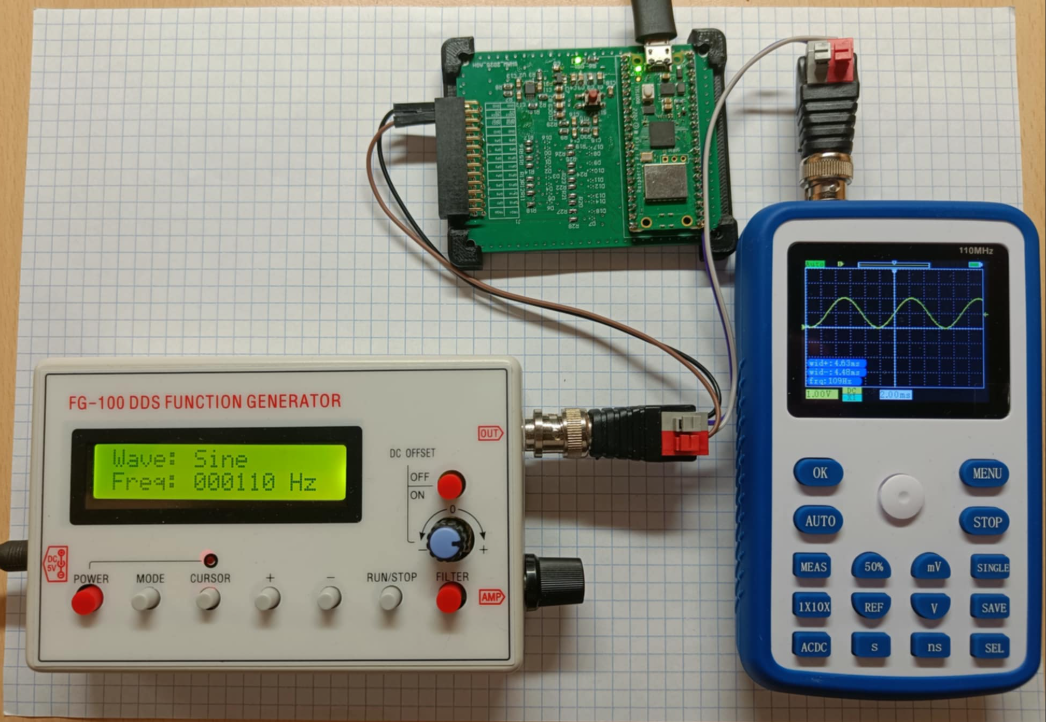
\includegraphics[width = \textwidth]{stanowisko_pomiarowe.png}
        \caption{Układ stanowiska pomiarowego}
        \label{fig:stanowisko_pomiarowe}
    \end{figure}

    W celu przeprowadzeniu testów działania systemu, które na wczesnym etapie projektu
    mogłyby się odbywać niezależnie od aplikacji graficznej, postanowiono napisać
    skrypt w języku Python, dzieki któremu możliwe było obserwowanie zebranych danych
    wysyłanych przez WIFI do komputera. Widok aplikacji przedstawiono poniżej.
    
    \begin{figure}[H]
        \centering
        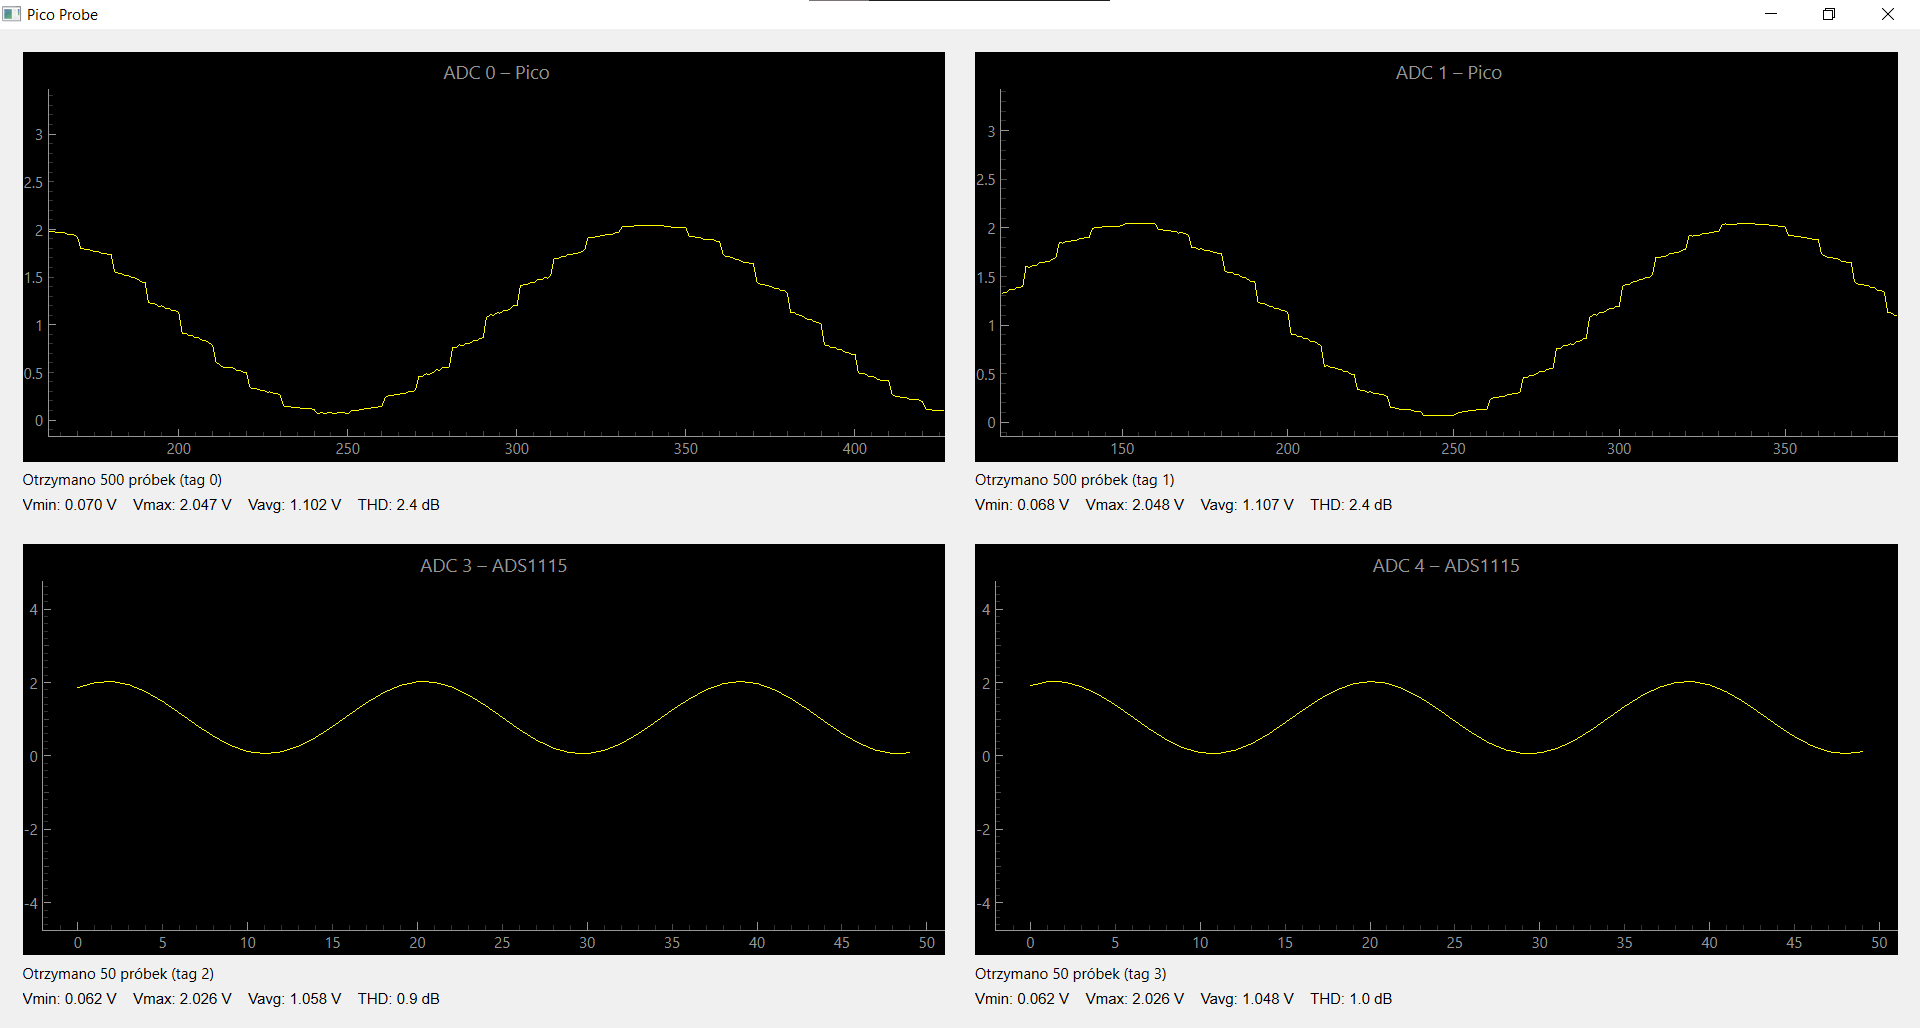
\includegraphics[width = \textwidth]{Analog_track_2.png}
        \caption{Pomocnicza aplikacja do obserwowania przebiegów sygnałów analogowych}
        \label{fig:Analog_track_2}
    \end{figure}

\subsection{Testowanie działania analizatora sygnałów analogowych}
    Jednym z najważniejszych parametrów przy testowaniu układów takich jak oscyloskopy
    czy ogólnie analizatory sygnałów analogowych jest min. maksymalna częstotliwość
    sygnałów które wiernie mogą odwzorowywać. Częstotliwość ta wynika bezpośrednio z 
    twierdzenia o próbkowaniu Nyquista-Shannona:
    \[
    f_s \geq 2 f_{\max}
    \]

    W rzeczywistości jednak częstotliwość próbkowania powinna być większa niż 
    dwukrotność maksymalnej składowej częstotliwościowej sygnału, często podaje się ją
    jako:
    \[
    f_s \geq 2.5 f_{\max}
    \]
    lub nawet więcej.

    Podczas przeprowadzenia testów, kryterium badania jakości mierzonych sygnałów była wartość
    THD(dla 4 harmonicznych), którą definiuje się następująco:
    \[
    \mathrm{THD}_{dB} = 20 \log_{10} \left( \frac{
    \sqrt{
    \sum_{h=2}^{5} \left|X(h f_1)\right|^2
    }
    }{
    \left|X(f_1)\right|
    } \right)
    \]
    Jeżeli więc zniekształcenia osiągały duże wartości(małe THD, czyli dużą zawartość
    pozostałych harmonicznych względem podstawowej) stwierdzano, że dalsze zwiększanie częstotliwości nie ma sensu
    i kończono pomiar na niej. Zebrane wyniki pomiarów przedstawiono poniżej.

    \begin{table}[!ht]
        \centering
        \begin{tabular}{|c|>{\centering\arraybackslash}m{4cm}|>{\centering\arraybackslash}m{4cm}|}
            \hline
            \textbf{Nazwa przetwornika} &
            \makecell{\textbf{Teoretyczna maks.}\\\textbf{częstotliwość}} &
            \makecell{\textbf{Zmierzona maks.}\\\textbf{częstotliwość}} \\
            \hline
            ADS1115 & 250 Hz & 180 Hz \\
            \hline
            Pico ADC & 2.5 kHz & 250 Hz \\
            \hline
        \end{tabular}
        \caption{Wyniki testów analizatora sygnałów analogowych}
        \label{tab:freq_test_results}
    \end{table}

    \subsection{Zaobserwowane problemy z działaniem układu.}
    Jak można było to już wcześniej zauważyć(rys.~\ref{fig:Analog_track_2})
    wykres amplitudowy z ADC Pico jest mocno zniekształcony, jeszcze lepiej
    widać to na poniższej ilustracji.
     
    \begin{figure}[H]
        \centering
        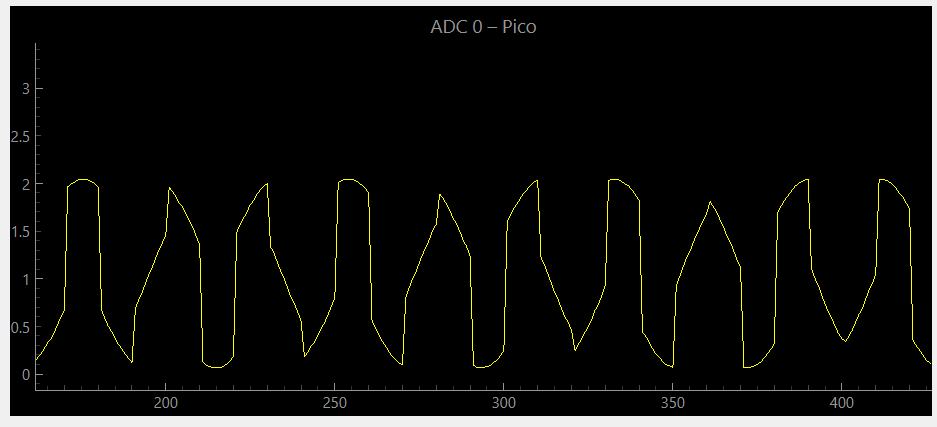
\includegraphics[width = \textwidth]{analog_distortion.png}
        \caption{Wstępnie przetworzony sygnał wyjściowy z ADC Pico}
        \label{fig:analog_distortion}
    \end{figure}

    Charakter wykresu nie jest spowodowany zbyt wysoką częstotliwością podawanego
    sygnału lecz skutkiem działania systemu. Duże zniekształcenia sygnału wynikają
    z transmisji I2C która z racji na bardzo sprzętowy charakter, jeżeli wystąpi blokuje
    cały rdzeń w skutek, czego to co zbiera ADC Pico jest mocno zniekształcone.
    Podczas projektowania układu podejmowano różne techniki niwelowania takiego zachowania tj.: 
    \begin{enumerate}
        \item Praca z I2C na przerwaniach z wykorzystaniem maszyny stanów.
        \item Wykorzystanie wbudowanej funkcjonalności ADS1115 która umożliwia zgłaszanie przez.
        przetwornik zdarzenia zakończenia konwersji przez co nie trzeba na nią czekać tracąc czas
        rdzenia.
    \end{enumerate}

    Innym pomysłem na rozwiązanie tego problemu było by zastosowanie innego przetwornika ADC wykorzystującego szybsze protokoły transmisji(np. SPI)
    lub inne topologie wewnętrznego ADC.

    Niestety ostatecznie nie udało się doprowadzić żadnej z wyżej wymienionych opcji do stanu
    który można by uznać za zadowalający, głównie ze względu na rosnącą złożoność sytemu kontrolno-pomiarowego
    którego dobrze działająca implementacja okazała się bardzo pracochłonna i skomplikowana.
    
    Dlatego właśnie maksymalna częstotliwość Pico ADC pomimo znacznie większego
    próbkowania ostatecznie okazała się niedużo większa niż znacznie wolniejszego ADS1115.  